\begin{enunciado}{\ejercicio}
  \begin{minipage}{0.5\textwidth}
    Dados los siguientes $z,\,w \en \complejos$ en el plano:
  \end{minipage}
  \begin{minipage}{0.5\textwidth}
    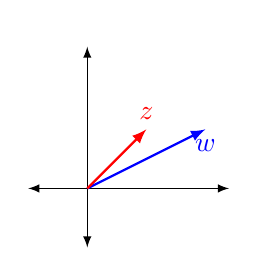
\begin{tikzpicture}[scale=1.5]
      % Draw the main coordinate axes
      \draw[latex-latex] (-0.5,0) -- (1.2,0) node[right] {$\re$};
      \draw[latex-latex] (0,-0.5) -- (0,1.2) node[above] {$\im$};

      \draw[blue,thick,-latex] (0,0) -- (1,{1/2}) node[right, below] {$w$};
      \draw[red,thick,-latex] (0,0) -- ({1/2},{1/2}) node[left, above] {$z$};
    \end{tikzpicture}
  \end{minipage}
  Representar en un gráfico aproximado los números complejos de cada inciso
  \begin{enumerate}[label=\roman*)]
    \begin{multicols}{3}
      \item $z, w, z + w \ytext z - w$
      \item $z, -z, 2z, \frac{1}{2}z, iz \ytext \conj{z}$
      \item $z, w, |z|,  |z + w| \ytext |\conj{w - z}|$.
    \end{multicols}
  \end{enumerate}
\end{enunciado}
\begin{center}
\begin{enumerate}[label=\roman*)]
  \item
        $$
          \begin{tikzpicture}[scale=3.5, every node/.style={font={\tiny}}, baseline=3cm]
            \draw[ultra thin, latex-latex] (-0.8,0) -- (1.6,0) node[below] {$\re$};
            \draw[ultra thin, latex-latex] (0,-0.5) -- (0,1.2) node[left] {$\im$};

            \draw[blue,thin,-latex,opacity=0.2] (0,0) -- (1,0.5) node[right, below] {$w$};
            \draw[red,thin,-latex,opacity=0.2] (0,0) -- (0.5,0.5) node[midway, yshift=1pt, xshift=-2pt]{$z$};

            \draw[magenta,-latex,thick] (0,0) -- (1.5,1) node[above] {$z+w$};
            \draw[cyan,-latex, thick] (0,0) -- (-0.5,0) node[midway, yshift = -3pt] {$z-w$};
            \draw[blue,thin,-latex,opacity=0.2]  (0.5,0.5) -- ++(1,0.5) node[midway, yshift=4pt] {$w$};
            \draw[blue,thin,|-latex,opacity=0.2] (0.5,0.5) -- ++ (-1,-0.5) node[midway, yshift=5pt]{$-w$};
          \end{tikzpicture}
        $$

  \item
        $$
          \begin{tikzpicture}[scale=3.5, every node/.style={font={\tiny}}, baseline=3cm]
            \draw[ultra thin, latex-latex] (-1,0) -- (1.2,0) node[below] {$\re$};
            \draw[ultra thin, latex-latex] (0,-0.5) -- (0,1.2) node[left] {$\im$};

            \draw[red,thin,|-latex,opacity=0.2] (0,0) -- (0.5,0.5) node[left]{$z$};

            \draw[magenta,thick,-latex] (0,0) -- (-0.5,-0.5) node[left]{$-z$};
            \draw[cyan,thick,-latex] (0,0) -- (1,1) node[right]{$2z$};
            \draw[yellow!70!black,thick,-latex] (0,0) -- (0.25,0.25) node[midway, yshift=-3pt, xshift=5pt]{$\frac{1}{2}z$};
            \draw[green,thick,-latex] (0,0) -- (-0.5,0.5) node[left]{$iz$};
            \draw[-latex,thin] (0.25, 0.25) arc (45:135:{sqrt(2)/4}) node[midway, yshift=4pt]{$90^{\circ}$};
            \draw[violet,thick,-latex] (0,0) -- (0.5,-0.5) node[right]{$\conj{z}$};
          \end{tikzpicture}
        $$

  \item
        $$
          \begin{tikzpicture}[scale=3.5, every node/.style={font={\tiny}}, baseline=3cm]
            \draw[ultra thin, latex-latex] (-.25,0) -- (2.2,0) node[below] {$\re$};
            \draw[ultra thin, latex-latex] (0,-.25) -- (0,0.75) node[left] {$\im$};

            \draw[blue,thin,-latex,opacity=0.2] (0,0) -- (1,0.5) node[right, below] {$w$};
            \draw[red,thin,-latex,opacity=0.2] (0,0) -- (0.5,0.5) node[midway, yshift=1pt, xshift=-2pt]{$z$};

            \draw[Cerulean, thick, -latex] (0,0) -- ({1/sqrt(2)},0) node[yshift= 5pt]{$|z|$};
            \draw[violet, -latex, thick] (0,0) -- ({sqrt(1.5*1.5 + 1)},0) node[yshift = 5pt] {$|z+w|$};
            \draw[green, -latex, thick] (0,0) -- (0.5,0) node[yshift = -5pt] {$|w - z|$};
          \end{tikzpicture}
        $$
\end{enumerate}

\begin{aportes}
  \item \aporte{\dirRepo}{naD GarRaz \github}
\end{aportes}
